\newpage
\section{More about Quasi Particles}
\subsection{A soluble fermion system: The pure Hartree model}
Imagine that we have an N-fermion system with no external potential, and with a pure forward-scattering interaction between particles of the form
$$V_{k l m n}=V_{k l k l} \delta_{m k} \delta_{n l}$$
Placing this in the general Hamiltonian yields
\begin{equation}H=\sum_{k} \epsilon_{k} c_{k}^{\dagger} c_{k}+\frac{1}{2} \sum_{k i} V_{k l k l} c_{l}^{\dagger} c_{k}^{\dagger} c_{k} c_{l}
\label{pure-hartree-hamil}
\end{equation}
This model H will be called the 'pure Hartree' Hamiltonian, since, as we shall show, the only terms in it are those giving rise to the 'Hartree effective field'. Our object here is to get a solution to the problem in the form of 
\begin{equation}H^{\prime}=E_{0}+\sum_{q} \epsilon_{q}^{\prime} A_{q}^{\dagger} A_{q}+\underbrace{f\left(\ldots, A_{q}, \ldots, A_{q}^{\dagger}, \ldots\right)}_{\text {small }}\end{equation}
from
\begin{equation}H=\sum_{k} \epsilon_{k} c_{k}^{\dagger} c_{k}+\frac{1}{2} \sum_{k, l, m, n} V_{k l m n} c_{l}^{\dagger} c_{k}^{\dagger} c_{m} c_{n}\end{equation},
i.e., \bluep{the ground state energy plus a set of approximately independent elementary excitations above the ground state.} We do this by the straightforward diagrammatic method.

The interaction (\ref{pure-hartree-hamil}) has only the simple forms
\begin{equation}
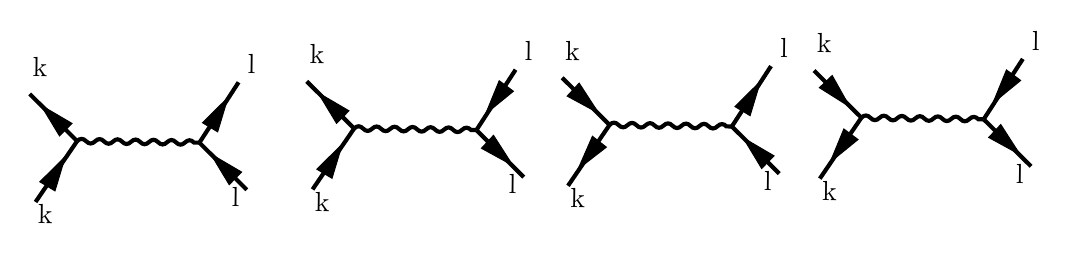
\begin{tikzpicture}[x=0.65pt,y=0.65pt,yscale=-1,xscale=1]
%uncomment if require: \path (0,705); %set diagram left start at 0, and has height of 705

%Straight Lines [id:da613823184290475] 
\draw [line width=1.5]    (69.46,540.64) .. controls (71.15,538.99) and (72.81,539.01) .. (74.46,540.7) .. controls (76.11,542.39) and (77.77,542.41) .. (79.46,540.77) .. controls (81.15,539.12) and (82.81,539.14) .. (84.46,540.83) .. controls (86.11,542.52) and (87.77,542.54) .. (89.46,540.9) .. controls (91.15,539.25) and (92.81,539.27) .. (94.46,540.96) .. controls (96.11,542.65) and (97.77,542.67) .. (99.46,541.03) .. controls (101.15,539.38) and (102.81,539.4) .. (104.46,541.09) .. controls (106.11,542.78) and (107.77,542.8) .. (109.46,541.15) .. controls (111.15,539.51) and (112.81,539.53) .. (114.46,541.22) .. controls (116.11,542.91) and (117.77,542.93) .. (119.46,541.28) .. controls (121.15,539.64) and (122.81,539.66) .. (124.45,541.35) .. controls (126.1,543.04) and (127.76,543.06) .. (129.45,541.41) .. controls (131.14,539.77) and (132.8,539.79) .. (134.45,541.48) -- (137.45,541.52) -- (137.45,541.52) ;
%Straight Lines [id:da6353755682299548] 
\draw [line width=1.5]    (43.13,514.46) -- (69.46,540.64) ;
%Straight Lines [id:da6254606220772768] 
\draw [line width=1.5]    (137.45,541.52) -- (163.78,567.69) ;
%Straight Lines [id:da5480869883300985] 
\draw [line width=1.5]    (69.46,540.64) -- (46.35,574.51) ;
%Straight Lines [id:da49445752084181116] 
\draw [line width=1.5]    (159.22,507.96) -- (137.45,541.52) ;
%Shape: Triangle [id:dp022384072825595847] 
\draw  [fill={rgb, 255:red, 0; green, 0; blue, 0 }  ,fill opacity=1 ] (49.47,520.82) -- (66.54,530.81) -- (59.69,537.75) -- cycle ;
%Shape: Triangle [id:dp5669679661948073] 
\draw  [fill={rgb, 255:red, 0; green, 0; blue, 0 }  ,fill opacity=1 ] (143.8,547.87) -- (160.86,557.87) -- (154.01,564.81) -- cycle ;
%Shape: Triangle [id:dp23872151900315752] 
\draw  [fill={rgb, 255:red, 0; green, 0; blue, 0 }  ,fill opacity=1 ] (153.28,516.53) -- (147.58,535.46) -- (139.22,530.44) -- cycle ;
%Shape: Triangle [id:dp5504301680867448] 
\draw  [fill={rgb, 255:red, 0; green, 0; blue, 0 }  ,fill opacity=1 ] (62.85,549.36) -- (57.15,568.3) -- (48.79,563.27) -- cycle ;
%Straight Lines [id:da6839577763606166] 
\draw [line width=1.5]    (223.46,533.64) .. controls (225.15,531.99) and (226.81,532.01) .. (228.46,533.7) .. controls (230.11,535.39) and (231.77,535.41) .. (233.46,533.77) .. controls (235.15,532.12) and (236.81,532.14) .. (238.46,533.83) .. controls (240.11,535.52) and (241.77,535.54) .. (243.46,533.9) .. controls (245.15,532.25) and (246.81,532.27) .. (248.46,533.96) .. controls (250.11,535.65) and (251.77,535.67) .. (253.46,534.03) .. controls (255.15,532.38) and (256.81,532.4) .. (258.46,534.09) .. controls (260.11,535.78) and (261.77,535.8) .. (263.46,534.15) .. controls (265.15,532.51) and (266.81,532.53) .. (268.46,534.22) .. controls (270.11,535.91) and (271.77,535.93) .. (273.46,534.28) .. controls (275.15,532.64) and (276.81,532.66) .. (278.45,534.35) .. controls (280.1,536.04) and (281.76,536.06) .. (283.45,534.41) .. controls (285.14,532.77) and (286.8,532.79) .. (288.45,534.48) -- (291.45,534.52) -- (291.45,534.52) ;
%Straight Lines [id:da9240174823017793] 
\draw [line width=1.5]    (197.13,507.46) -- (223.46,533.64) ;
%Straight Lines [id:da42566261374485415] 
\draw [line width=1.5]    (291.45,534.52) -- (317.78,560.69) ;
%Straight Lines [id:da016054446409110024] 
\draw [line width=1.5]    (223.46,533.64) -- (200.35,567.51) ;
%Straight Lines [id:da7774023230842375] 
\draw [line width=1.5]    (313.22,500.96) -- (291.45,534.52) ;
%Shape: Triangle [id:dp3043226594104913] 
\draw  [fill={rgb, 255:red, 0; green, 0; blue, 0 }  ,fill opacity=1 ] (203.47,513.82) -- (220.54,523.81) -- (213.69,530.75) -- cycle ;
%Shape: Triangle [id:dp9365361434860027] 
\draw  [fill={rgb, 255:red, 0; green, 0; blue, 0 }  ,fill opacity=1 ] (311.63,554.14) -- (294.29,544.63) -- (300.94,537.5) -- cycle ;
%Shape: Triangle [id:dp13172855405910544] 
\draw  [fill={rgb, 255:red, 0; green, 0; blue, 0 }  ,fill opacity=1 ] (296.64,525.44) -- (304.12,507.14) -- (311.96,512.94) -- cycle ;
%Shape: Triangle [id:dp6150273572328407] 
\draw  [fill={rgb, 255:red, 0; green, 0; blue, 0 }  ,fill opacity=1 ] (216.85,542.36) -- (211.15,561.3) -- (202.79,556.27) -- cycle ;
%Straight Lines [id:da10558670890674016] 
\draw [line width=1.5]    (505.46,527.64) .. controls (507.15,525.99) and (508.81,526.01) .. (510.46,527.7) .. controls (512.11,529.39) and (513.77,529.41) .. (515.46,527.77) .. controls (517.15,526.12) and (518.81,526.14) .. (520.46,527.83) .. controls (522.11,529.52) and (523.77,529.54) .. (525.46,527.9) .. controls (527.15,526.25) and (528.81,526.27) .. (530.46,527.96) .. controls (532.11,529.65) and (533.77,529.67) .. (535.46,528.03) .. controls (537.15,526.38) and (538.81,526.4) .. (540.46,528.09) .. controls (542.11,529.78) and (543.77,529.8) .. (545.46,528.15) .. controls (547.15,526.51) and (548.81,526.53) .. (550.46,528.22) .. controls (552.11,529.91) and (553.77,529.93) .. (555.46,528.28) .. controls (557.15,526.64) and (558.81,526.66) .. (560.45,528.35) .. controls (562.1,530.04) and (563.76,530.06) .. (565.45,528.41) .. controls (567.14,526.77) and (568.8,526.79) .. (570.45,528.48) -- (573.45,528.52) -- (573.45,528.52) ;
%Straight Lines [id:da4301121902778472] 
\draw [line width=1.5]    (479.13,501.46) -- (505.46,527.64) ;
%Straight Lines [id:da8070089193956563] 
\draw [line width=1.5]    (573.45,528.52) -- (599.78,554.69) ;
%Straight Lines [id:da9369302080120971] 
\draw [line width=1.5]    (505.46,527.64) -- (482.35,561.51) ;
%Straight Lines [id:da6514758529059829] 
\draw [line width=1.5]    (595.22,494.96) -- (573.45,528.52) ;
%Shape: Triangle [id:dp46358512529050333] 
\draw  [fill={rgb, 255:red, 0; green, 0; blue, 0 }  ,fill opacity=1 ] (498.9,521.5) -- (482.16,510.96) -- (489.23,504.24) -- cycle ;
%Shape: Triangle [id:dp38044017958960863] 
\draw  [fill={rgb, 255:red, 0; green, 0; blue, 0 }  ,fill opacity=1 ] (593.63,548.14) -- (576.29,538.63) -- (582.94,531.5) -- cycle ;
%Shape: Triangle [id:dp28303426408257704] 
\draw  [fill={rgb, 255:red, 0; green, 0; blue, 0 }  ,fill opacity=1 ] (578.64,519.44) -- (586.12,501.14) -- (593.96,506.94) -- cycle ;
%Shape: Triangle [id:dp44406046766962526] 
\draw  [fill={rgb, 255:red, 0; green, 0; blue, 0 }  ,fill opacity=1 ] (488.19,552.26) -- (495.71,533.97) -- (503.54,539.79) -- cycle ;
%Straight Lines [id:da7271479706009089] 
\draw [line width=1.5]    (365.46,531.64) .. controls (367.15,529.99) and (368.81,530.01) .. (370.46,531.7) .. controls (372.11,533.39) and (373.77,533.41) .. (375.46,531.77) .. controls (377.15,530.12) and (378.81,530.14) .. (380.46,531.83) .. controls (382.11,533.52) and (383.77,533.54) .. (385.46,531.9) .. controls (387.15,530.25) and (388.81,530.27) .. (390.46,531.96) .. controls (392.11,533.65) and (393.77,533.67) .. (395.46,532.03) .. controls (397.15,530.38) and (398.81,530.4) .. (400.46,532.09) .. controls (402.11,533.78) and (403.77,533.8) .. (405.46,532.15) .. controls (407.15,530.51) and (408.81,530.53) .. (410.46,532.22) .. controls (412.11,533.91) and (413.77,533.93) .. (415.46,532.28) .. controls (417.15,530.64) and (418.81,530.66) .. (420.45,532.35) .. controls (422.1,534.04) and (423.76,534.06) .. (425.45,532.41) .. controls (427.14,530.77) and (428.8,530.79) .. (430.45,532.48) -- (433.45,532.52) -- (433.45,532.52) ;
%Straight Lines [id:da7854992580693345] 
\draw [line width=1.5]    (339.13,505.46) -- (365.46,531.64) ;
%Straight Lines [id:da338940395062972] 
\draw [line width=1.5]    (433.45,532.52) -- (459.78,558.69) ;
%Straight Lines [id:da20114032104584845] 
\draw [line width=1.5]    (365.46,531.64) -- (342.35,565.51) ;
%Straight Lines [id:da47776944835115154] 
\draw [line width=1.5]    (455.22,498.96) -- (433.45,532.52) ;
%Shape: Triangle [id:dp9747602816540912] 
\draw  [fill={rgb, 255:red, 0; green, 0; blue, 0 }  ,fill opacity=1 ] (359.33,525.05) -- (341.95,515.63) -- (348.56,508.47) -- cycle ;
%Shape: Triangle [id:dp8973952534123313] 
\draw  [fill={rgb, 255:red, 0; green, 0; blue, 0 }  ,fill opacity=1 ] (439.8,538.87) -- (456.86,548.87) -- (450.01,555.81) -- cycle ;
%Shape: Triangle [id:dp7615505790794537] 
\draw  [fill={rgb, 255:red, 0; green, 0; blue, 0 }  ,fill opacity=1 ] (449.28,507.53) -- (443.58,526.46) -- (435.22,521.44) -- cycle ;
%Shape: Triangle [id:dp860067401387033] 
\draw  [fill={rgb, 255:red, 0; green, 0; blue, 0 }  ,fill opacity=1 ] (348.02,556.14) -- (355.95,538.02) -- (363.64,544.01) -- cycle ;

% Text Node
\draw (46.35,574.51) node [anchor=north west][inner sep=0.75pt]  [rotate=-0.74] [align=left] {k};
% Text Node
\draw (43.41,492.46) node [anchor=north west][inner sep=0.75pt]  [rotate=-0.74] [align=left] {k};
% Text Node
\draw (154.01,564.81) node [anchor=north west][inner sep=0.75pt]  [rotate=-0.74] [align=left] {l};
% Text Node
\draw (162.97,490.91) node [anchor=north west][inner sep=0.75pt]  [rotate=-0.74] [align=left] {l};
% Text Node
\draw (200.35,567.51) node [anchor=north west][inner sep=0.75pt]  [rotate=-0.74] [align=left] {k};
% Text Node
\draw (197.41,485.46) node [anchor=north west][inner sep=0.75pt]  [rotate=-0.74] [align=left] {k};
% Text Node
\draw (308.01,557.81) node [anchor=north west][inner sep=0.75pt]  [rotate=-0.74] [align=left] {l};
% Text Node
\draw (316.97,483.91) node [anchor=north west][inner sep=0.75pt]  [rotate=-0.74] [align=left] {l};
% Text Node
\draw (482.35,561.51) node [anchor=north west][inner sep=0.75pt]  [rotate=-0.74] [align=left] {k};
% Text Node
\draw (479.41,479.46) node [anchor=north west][inner sep=0.75pt]  [rotate=-0.74] [align=left] {k};
% Text Node
\draw (590.01,551.81) node [anchor=north west][inner sep=0.75pt]  [rotate=-0.74] [align=left] {l};
% Text Node
\draw (598.97,477.91) node [anchor=north west][inner sep=0.75pt]  [rotate=-0.74] [align=left] {l};
% Text Node
\draw (342.35,565.51) node [anchor=north west][inner sep=0.75pt]  [rotate=-0.74] [align=left] {k};
% Text Node
\draw (339.41,483.46) node [anchor=north west][inner sep=0.75pt]  [rotate=-0.74] [align=left] {k};
% Text Node
\draw (450.01,555.81) node [anchor=north west][inner sep=0.75pt]  [rotate=-0.74] [align=left] {l};
% Text Node
\draw (458.97,481.91) node [anchor=north west][inner sep=0.75pt]  [rotate=-0.74] [align=left] {l};


\end{tikzpicture}
\end{equation}
Hence the only graphs occurring in the series for the ground state energy are 
\begin{equation}
    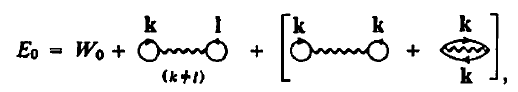
\includegraphics[width=0.8\textwidth]{screenshots/pure-hartree-diam.PNG}
    \label{pure-hartree-diam}
\end{equation}
Note that \textbf{the propagator lines in these diagrams are all hole lines. Also the diagrams in brackets violate the exclusion principle since there are simultaneously two hole lines in state $\mathbf{k}$}.
\begin{equation}E_{0}=\sum_{k<k=7} \epsilon_{k}+\frac{1}{2} \sum_{\substack{k, l<k_F\\\mathbf{k}\neq\mathbf{l}}}^{\prime} V_{k l k l}
\label{pure-hartree-E0}
\end{equation}
The $\mathbf{k=l}$ graphs cancel because of the fermion loop in bubble diagram.

Now let us get the quasi particle energies, $\epsilon_k^{\prime}$, from the poles of the Green's function. In this case, the propagator is given exactly by the sum over just the bubble graphs:
\begin{equation}
    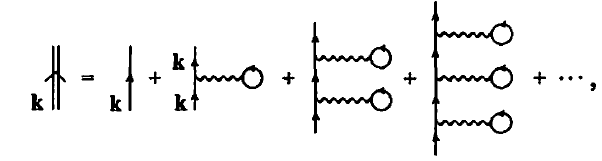
\includegraphics[width=0.8\textwidth]{screenshots/pure-hartree-diam-series.PNG}
    \label{pure-hartree-diam-series}
\end{equation}
Series (\ref{pure-hartree-diam-series}) was summed and gives the result for quasi particle energy, as shown in chapter 4,
\begin{equation}\begin{array}{l}
\epsilon_{k}^{\prime}=\epsilon_{k}+\sum_{l<k_F} V_{k l k l}, \quad k>k_{F} \\
\tau_{k}=\infty
\end{array}
\label{pure-hartree-E-particle}
\end{equation}
In the case of quasi holes we just sum
\begin{equation}
    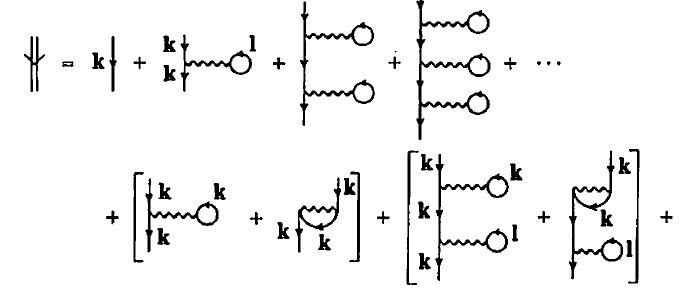
\includegraphics[width=0.8\textwidth]{screenshots/pure-hartree-hole-diam-series.PNG}
    \label{pure-hartree-hole-diam-series}
\end{equation}
The bracketed diagrams cancel because of the fermion loop and we get the result:
\begin{equation}\begin{aligned}
&\epsilon_{k}^{\prime}=\epsilon_{k}+\sum_{l<k_{F}}{}^{\prime} V_{k l k l}, \quad k<k_{F}\\
&\tau_{k}=\infty
\end{aligned}
\label{pure-hartree-E-hole}
\end{equation}

Finally, we need the interaction between quasi particles ($f$-term in (\ref{pure-hartree-hamil})).This can be obtained from the various two-particle propagators. Consider the particle-particle propagator first. In the present case, this is given by the sum:
\begin{equation}
    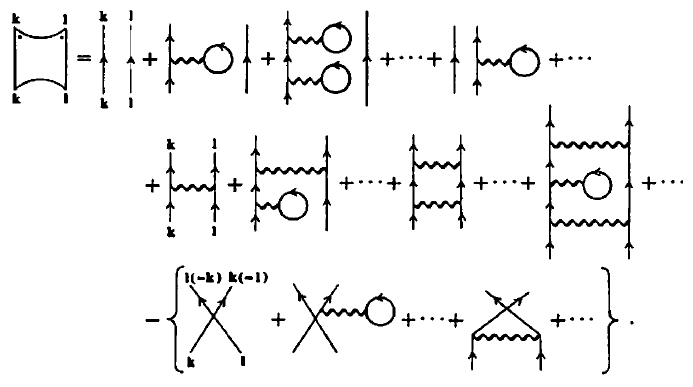
\includegraphics[width=0.8\textwidth]{screenshots/particle-particle-diam-series.PNG}
    \label{particle-particle-diam-series}
\end{equation}
The crossed "exchange" diagrams in the brackets in (\ref{particle-particle-diam-series}) contribute only when $\mathbf{k}=\mathbf{l}$. because the labels on the incoming and outgoing lines in each diagram must match those of $G_2$ on the left. \redp{\textbf{Since these diagrams are negative, they cancel all the uncrossed diagrams when $\mathbf{k=l}$, so $G_2=0$ for $\mathbf{k=l}$}}.

We can greatly simplify (\ref{particle-particle-diam-series}) in the following way:
Consider the diagram subset consisting of more and more bubbles inserted into the first propagator,i.e.,:
\begin{equation}
    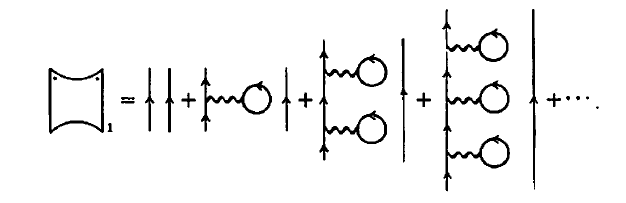
\includegraphics[width=0.8\textwidth]{screenshots/particle-particle-diam-series-2.PNG}
    \label{particle-particle-diam-series-2}
\end{equation}
This can be summed as:
\begin{equation}
    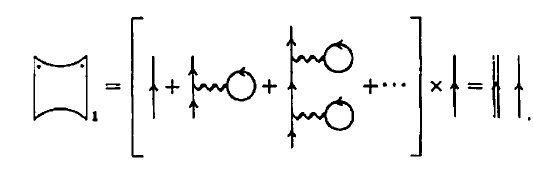
\includegraphics[width=0.8\textwidth]{screenshots/particle-particle-diam-series-3.PNG}
\end{equation}
Similarly, we sum over all bubble insertions in all bare propagators, leading to a sum in which all propagators are clothed,\redp{i.e.,} in which all propagators are the quasi particle propagators:
\begin{equation}
    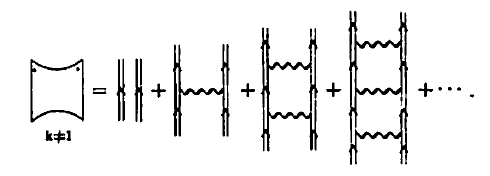
\includegraphics[width=0.8\textwidth]{screenshots/particle-particle-diam-series-4.PNG}
\end{equation}
In this form, we can see that the quasi particle interaction is:$V=V_{klkl}(l\neq k), V=0(l=k)$. Similar arguments applied to the particle-hole and hole-hole propagators yield this same interaction.

We can now combine these results into a Hamiltonian of form (\ref{pure-hartree-hamil}). The expressions for $E_0$ and $\epsilon_q^{\prime}$ are in (\ref{pure-hartree-E0}),(\ref{pure-hartree-E-particle}), and (\ref{pure-hartree-E-hole}). The interaction term $f$ in (\ref{pure-hartree-hamil}) will have the form
$$H_{1}=\frac{1}{2} \sum_{k, l, m, n} V_{k l m n} c^{\dagger}, c_{k}^{\dagger} c_{m} c_{n}$$
since the quasi particles here are fermions.

Letting $A_{k}^{\dagger}, A_{k}, B_{k}^{\dagger}, B_{k},$ be the quasi particle and quasi hole operators we find
\begin{equation}\begin{aligned}
H^{\prime}=[&\sum_{k<k_{F}} \epsilon_{k}+\frac{1}{2} \sum_{k,l<k_F}^{\prime} V_{k l k l}]+\\
&+\sum_{k<k_{F}}\left(\epsilon_{k}+\sum_{l<k_{p}} V_{k l k l}\right) A_{k}^{\dagger} A_{k}-\sum_{k<k_{F}}\left(\epsilon_{k}+\sum_{l<k_{F}}^{\prime} V_{klkl}\right) B_{k}^{\dagger} B_{k}+\\
&+\frac{1}{2} \sum_{l,k>k_{F}}^{\prime} V_{kl k l} A_{l}^{\dagger} A_{k}^{\dagger} A_{k} A_{l}-\sum_{\substack{k>k_{F}\\l<k_F}} V_{k l k l} B_{l}^{\dagger} A_{k}^{\dagger} A_{k} B_{l}+\\
&+\frac{1}{2} \sum_{\substack{k<k_F\\l<k_F}}^{\prime} V_{klkl} B_{l}^{\dagger} B_{k}^{\dagger} B_{k} B_{l}
\end{aligned}\end{equation}
Observe that in the particle-particle and hole-hole interaction terms, \textbf{it is necessary to put in a factor $\frac{1}{2}$ to avoid counting interactions twice when we sum freely over $\mathbf{k}$ and $\mathbf{l}$.} Note that the $(-)$ sign in the $B_{k}^{1} B_{k}$ term is put in because the hole energies (and therefore the quasi hole energies) are negative. The (-) in the $B_{l}^{t} A_{k}^{1} A_{k} B_{l}$ term occurs for the following reason: \bluep{The energy of a quasi particle in, say, state $k_1>k_F$, includes interactions with all particles in the filled Fermi sea. But if there is a hole in, say, state $l_1<k_F$, then the corresponding energy,$V_{k_1l_1k_1l_1}$ does not exist, and should be subtracted from the quasi particle energy. The term $-V_{k_1l_1k_1l_1}B_{l_1}^{\dagger}A_{k_1}^{\dagger}A_{k_1}B_{l_1}$  takes care of this substraction.}

\subsection{Crude calculation of quasi particle lifetime}
We mentioned that \redp{the quasi particle picture breaks down if the energy is two far away from the Fermi energy.} In a Fermi system, since one deals with particle-like excitation above $\epsilon_F^{\prime}$ (the Fermi energy of the interacting system), and hole-like ones below, the criterion is taken relative to the Fermi energy, i.e.:
\begin{equation}\frac{1}{\tau_{k}} \ll \epsilon_{k}^{\prime}-\epsilon_{F}^{\prime}\end{equation}
In the pure Hartree model,$\tau_k=\infty$, so this is satisfied for any $k$. But this is not true in general. In fact, we are now going to show that in most Fermi systems the quasi particle lifetime obeys
\begin{equation}\frac{1}{\tau_{k}} \propto\left(\epsilon_{k}^{\prime}-\epsilon_{F}^{\prime}\right)^{2}
\label{lifetime-criterion}
\end{equation}
Here we will give a crude quasi-proof of (\ref{lifetime-criterion}).

\bluep{The lifetime of a quasi particle in momentum state $\mathbf{k}$ will be the \textbf{inverse of the transition probability per second that the quasi particle will be scattered out of state $\mathbf{k}$ by collisions with other quasi particles}.} Let us pretend that quasi particle collisions are like those between real particles (they are not, actually, since quasi particles can have a 'retarded', i.e., time-dependent, interaction even when the bare particles interact instantaneously) and calculate the transition probability out of state $\mathbf{k}_1$ for a particle in state $\mathbf{k}_1$, where $|\mathbf{k}_1|\geq k_F$. In a typical interaction, the particle will collide with a particle in state $|\mathbf{k}_2|\leq k_F$ and final state will be a particle in $\mathbf{k}_3$ and $\mathbf{k}_4$, where
\begin{equation}\mathbf{k}_{4}=\mathbf{k}_{1}+\mathbf{k}_{2}-\mathbf{k}_{3}\end{equation}
The transition probability is
\begin{equation}W_{k_{1}} \propto \int d^{3} k_{2} \int d^{3} k_{3}\left|V_{k_{3}, k_{1}+k_{2}-k_{3}, k_{1}, k_{2}}\right|^{2}
\label{crude-quasi-interaction-probability}
\end{equation}
To evaluate (\ref{crude-quasi-interaction-probability}) we note that by the Pauli principle all states under $k_F$ are occupied so that \begin{equation}\left|\mathbf{k}_{3}\right| \geqslant k_{F}, \quad\left|\mathbf{k}_{4}\right| \geqslant k_{F}
\label{crude-proof-1}
\end{equation}
by conservation of energy,
\begin{equation}k_{1}^{2}+k_{2}^{2}=k_{3}^{2}+k_{4}^{2}
\label{crude-proof-2}
\end{equation}
The equations above imply that 
\begin{equation}k_{1}^{2}+k_{2}^{2} \geqslant 2 k_{F}^{2}
\label{crude-proof-3}
\end{equation}
Consider first the limiting case when $\left|\mathbf{k}_{1}\right|=k_{F} .$ Then by (\ref{crude-proof-3})$, k_{2}^{2} \geqslant k_{F}^{2} .$ But since $\left|\mathbf{k}_{2}\right| \leqslant k_{F},$ this implies $\left|\mathbf{k}_{2}\right|=k_{F}$. Similarly, $\left|\mathbf{k}_{3}\right|=\left|\mathbf{k}_{4}\right|=k_{F} .$ \textbf{That is, all momenta lie on the Fermi sphere.} Suppose now that $\left|\mathbf{k}_{1}\right|=k_{F}+\delta$ where $k_{F} \gg \delta>0 .$ Then by (\ref{crude-proof-3}) $,\left|\mathbf{k}_{2}\right| \geqslant k_{F}-\delta .$ Similarly, since $\left|\mathbf{k}_{2}\right| \leqslant k_{F},$ we have that in order to satisfy (\ref{crude-proof-2}), $\left|\mathbf{k}_{\mathbf{3}}\right|,\left|\mathbf{k}_{4}\right|$ must be less than $k_{F}+\delta .$ Hence all momenta lie in a shell of thickness $\delta=\left|\mathbf{k}_{1}\right|-k_{F}$ around the Fermi sphere. Assuming there's nothing peculiar about the behaviour of $V$, the integral over the $\mathbf{k}_{2}$ -shell gives a factor $\propto 4 \pi k_{F}^{2}\left(\left|\mathbf{k}_{1}\right|-k_{F}\right),$ and the same for the $\mathbf{k}_{3}$ -shell, so
\begin{equation}W_{k_{1}} \propto\left(\left|\mathbf{k}_{1}\right|-k_{F}\right)^{2}\end{equation}
But
\begin{equation}\begin{aligned}
\epsilon_{k_{1}}-\epsilon_{p} \propto\left(k_{1}^{2}-k_{F}^{2}\right) &=\left(\left|\mathbf{k}_{1}\right|-k_{P}\right)\left(\left|\mathbf{k}_{1}\right|+k_{F}\right) \\
& \approx 2 k_{F}\left(\left|\mathbf{k}_{1}\right|-k_{F}\right)
\end{aligned}\end{equation}
Whence
\begin{equation}\frac{1}{\tau_{k}}=W_{k} \propto\left(\epsilon_{k}-\epsilon_{F}\right)^{2}\end{equation}

\subsection{General form of quasi particle propagator}